\documentclass[ 12pt ]{article}

\usepackage{amsmath}
\usepackage{amssymb}
\usepackage{cancel}
\usepackage{tikz}

\begin{document}

% title page
\title{Homework 1}
\author{Landon Fox}
\date{February 5, 2020}

\begin{flushleft}
Landon Fox \\
STAT 461 \\
Section 1001 \\
February 5, 2020
\end{flushleft}
\begin{center}
Homework 1
\end{center}

\section{2.2.2}
\begin{flalign}
A &= \{\, (r,b,g) : r+b+g=5,\, r,b,g\, \epsilon\, \{1,2,3,4,5,6\}\, \} \\
A &= \{\, (1,1,3),\, (1,2,2),\, (1,3,1),\, (2,1,2),\, (2,2,1),\, (3,1,1)\, \}
\end{flalign}

\section{2.2.10}
Assuming the darts can only land on the given target
\subsection{a}
\begin{flalign}
S_1 &= \{\, (1,1),\, (1,2),\, (1,4),\, (2,1),\, (2,2),\, (2,4),\, (4,1),\, (4,2),\, (4,4)\, \}
\end{flalign}

\subsection{b}
\begin{flalign}
S_2 &= \{\, 2,\, 3,\, 4,\, 5,\, 6,\, 8\, \}
\end{flalign}
\newpage

% problem 2.2.20 a
\section{2.2.20}

\subsection{a}
\begin{flalign}
A^c \cap B \cap C
\end{flalign}
\begin{center}
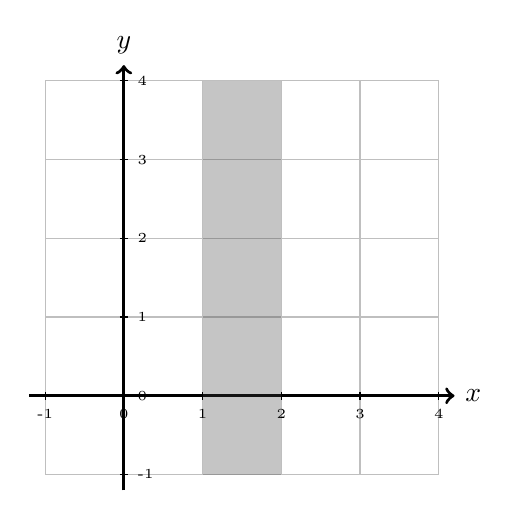
\begin{tikzpicture}
    \draw[gray!50, thin] (-1,-1) grid (4,4);
    \draw[very thick,->] (-1.2,0) -- (4.2,0) node[right] {$x$};
    \draw[very thick,->] (0,-1.2) -- (0,4.2) node[above] {$y$};

    \foreach \x in {-1,...,4} \draw (\x,0.05) -- (\x,-0.05) node[below] {\tiny\x};
    \foreach \y in {-1,...,4} \draw (-0.05,\y) -- (0.05,\y) node[right] {\tiny\y};

    \fill[black!50!gray,opacity=0.3] (1,-1) -- (1,4) -- (2,4) -- (2,-1) -- cycle;
\end{tikzpicture}
\end{center}

% problem 2.2.20 d
\subsection{d}
\begin{flalign}
((A \cup B) \cap C^c)^c
\end{flalign}
\begin{center}
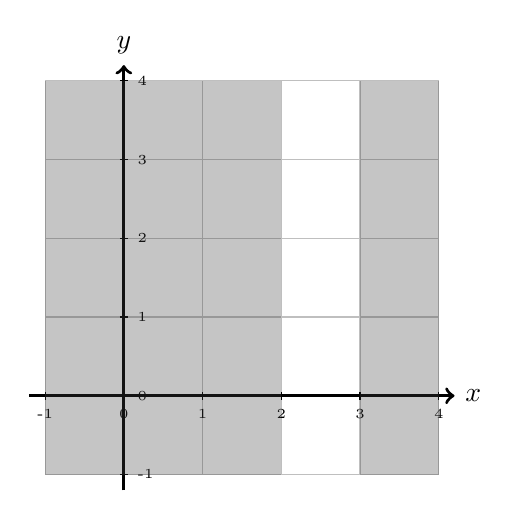
\begin{tikzpicture}
    \draw[gray!50, thin] (-1,-1) grid (4,4);
    \draw[very thick,->] (-1.2,0) -- (4.2,0) node[right] {$x$};
    \draw[very thick,->] (0,-1.2) -- (0,4.2) node[above] {$y$};

    \foreach \x in {-1,...,4} \draw (\x,0.05) -- (\x,-0.05) node[below] {\tiny\x};
    \foreach \y in {-1,...,4} \draw (-0.05,\y) -- (0.05,\y) node[right] {\tiny\y};

    \fill[black!50!gray,opacity=0.3] (-1,-1) -- (-1,4) -- (2,4) -- (2,-1) -- cycle;
    \fill[black!50!gray,opacity=0.3] (3,-1) -- (3,4) -- (4,4) -- (4,-1) -- cycle;
\end{tikzpicture}
\end{center}

\section{2.2.26}

\subsection{d}
\begin{flalign}
(A\cap B^c\cap C^c)\cup(A^c\cap B\cap C^c)\cup(A^c\cap B^c\cap C)
\end{flalign}

\subsection{e}
\begin{flalign}
((A\cap B)\cup(A\cap C)\cup(B\cap C))\cap(A^c\cup B^c\cup C^c)
\end{flalign}

\section{2.3.2}
Know:
\begin{flalign}
P(A) &= 0.4 \\
P(B) &= 0.5 \\
P(A \cap B) &= 0.1
\end{flalign}
Find:
\begin{flalign}
P(A\cup B - A \cap B)
\end{flalign}
\begin{center}
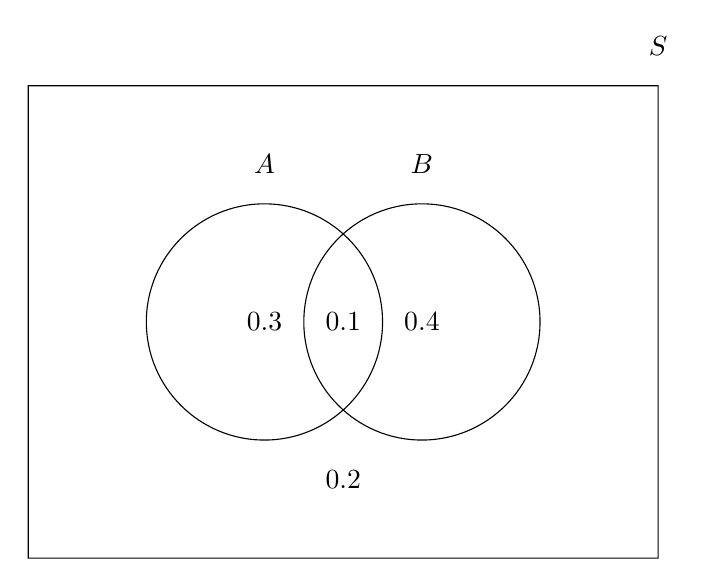
\begin{tikzpicture}[fill=gray]
\draw (-1,0) circle (1.5) (0,1)
      (1,0) circle (1.5) (1,1)
      (-4,-3) rectangle (4,3)
      (4,3.5) node {$S$}
      (-1,2) node {$A$}
      (1,2) node {$B$}
      (-1,0) node {$0.3$}
      (1,0) node {$0.4$}
      (0,0) node {$0.1$}
      (0,-2) node {$0.2$};
\end{tikzpicture}
\end{center}
\begin{flalign}
P(A\cup B - A \cap B) &= (P(A) - P(A\cap B)) + (P(B) - P(A\cap B)) \\
&= (0.4-0.1)+(0.5-0.1) \\
&= 0.7
\end{flalign}

\section{2.3.5}
Does:
\begin{flalign}
P(A_1\cup A_2\cup A_3) =\frac{1}{2} \\
A_i: the\; ith\; die\; landing\; on\; a\; six
\end{flalign}
The above statement is not true because it does not account for mutual inclusion.
For instance, if both die one and two land on a six, their events are being double counted.
\begin{flalign}
P(A_1\cup A_2\cup A_3) &= 1-P(A_1^c\cap A_2^c\cap A_3^c) \\
&= 1-P(A_1^c)\cdot P(A_2^c)\cdot P(A_3^c) \\
&=1-\frac{5}{6} \cdot \frac{5}{6} \cdot \frac{5}{6} \\
&= \frac{191}{216}
\end{flalign}
\newpage

\section{2.3.10}
Given:
\begin{flalign}
S:\; &[1,24]\cap \mathbb{Z} \\
A:\; &\{\, x:2|x, x\,\epsilon\, S\, \} \\
B:\; &\{\, x:3|x, x\,\epsilon\, S\, \}
\end{flalign}
Find:
\begin{flalign}
P(A\cup B)& \\
P(A\cup B)& = P(A) + P(B) - P(A\cap B) \\
& = \frac{\frac{24}{2}}{24} + \frac{\frac{24}{3}}{24} - \frac{\frac{24}{6}}{24} \\
& = \frac{1}{2} + \frac{1}{3} - \frac{1}{6} \\
& = \frac{2}{3}
\end{flalign}

\section{2.3.14}
Given:
\begin{flalign}
P(A) &= 0.2 \\
P(B) &= 0.1 \\
P(C) &= 0.3
\end{flalign}
Minimize:
\begin{flalign}
P((A\cup B\cup C)^c)
\end{flalign}
To minimize the given statement, we can rephrase it as a maximization of the elements in the sets
given the initial conditions. If we say A, B, and C are mutually exclusive, elements will not be counted twice; allowing all values to be unique.
Therefore, the probability of the unions could be maximized to the sum of the probabilities of each set, giving:
\begin{flalign}
P((A\cup B\cup C)^c) &= 1 - P(A) - P(B) - P(C) \\
&= 0.4
\end{flalign}
\newpage

\section{}
Given:
\begin{flalign}
P(A) &= \frac{1}{2} \\
P(B^c) &= \frac{1}{3}
\end{flalign}
Can A and B be disjoint? Explain. \\
Assuming A and B are disjoint:
\begin{flalign}
A\cap B = \phi \rightarrow &P(A)+P(B) \leq P(S) \\
&\frac{1}{2}+\frac{2}{3} \leq 1 \\
&\frac{7}{6} \nleqslant 1 \\
\therefore A\cap B \neq \phi
\end{flalign}
If A and B are disjoint, it would then imply that their sum of their probabilities would be less than that of the sample space.
Otherwise, there could be items that were counted twice and exceed the probability of the sample space; as shown above.

\end{document}
